\chapter{Setting up and maintaining \ReplicaNextLong{}}\label{ch:replica-next-setup}

This section applies to the \ReplicaNextLong{} dashboard shown in \autoref{fig:next-hardware}.

\begin{figure}[htbp]
    \centering
    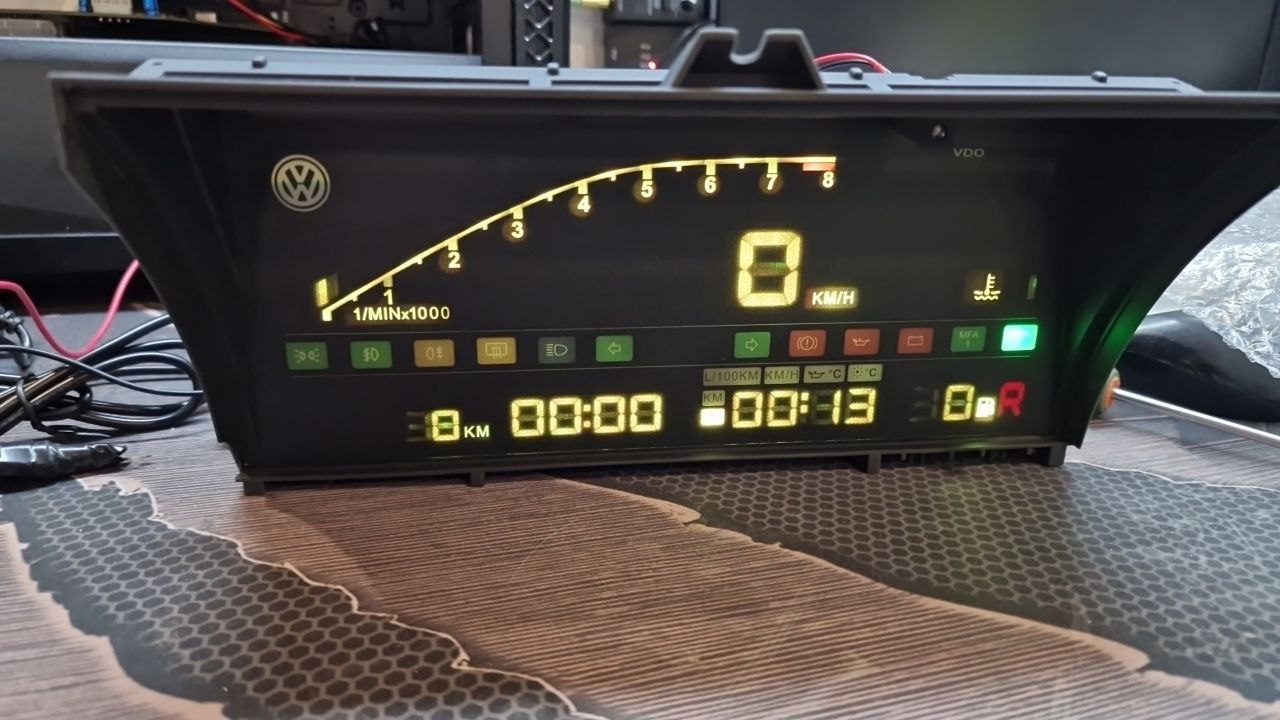
\includegraphics[width=0.6\textwidth]{digifiz_manual/image019.png}
    \caption{\ReplicaNextLong{} dashboard assembly.}
    \label{fig:next-hardware}
\end{figure}

\section{Panel handling}
\begin{itemize}
    \item The UV-printed polycarbonate faceplate must be protected from scratches and foreign objects. Significant damage requires replacement parts from PHOL-LABS Kft and is not treated as a warranty case.
    \item The real-time clock is configured via the Wi-Fi control panel. It resets whenever the permanent supply is disconnected.
\end{itemize}

\section{Wi-Fi control portal}
Configuration, data collection, and firmware management are performed through the embedded web application.
\begin{itemize}
    \item Connect to the dashboard's Wi-Fi access point. Disable mobile data and join \texttt{Digifiz\_AP} (password \texttt{87654321}); some revisions advertise \texttt{PHOL-LABS2} with the same password.
    \item The default IP address is \texttt{192.168.4.1}. If the dashboard is configured to join another network, scan the subnet for an address ending in \texttt{.32} using an IP tools application.
    \item The portal contains five tabs: \emph{WiFi}, \emph{Control}, \emph{Settings}, \emph{Colors}, and \emph{About} (\autoref{fig:next-control-tabs}). The Wi-Fi tab configures network settings and handles firmware uploads; the Control tab adjusts dashboard parameters; the Settings tab provides a structured editor for all firmware parameters; the Colors tab manages multi-segment colour schemes; the About tab lists author information.
\end{itemize}

\begin{figure}[htbp]
    \centering
    \begin{subfigure}{0.48\textwidth}
        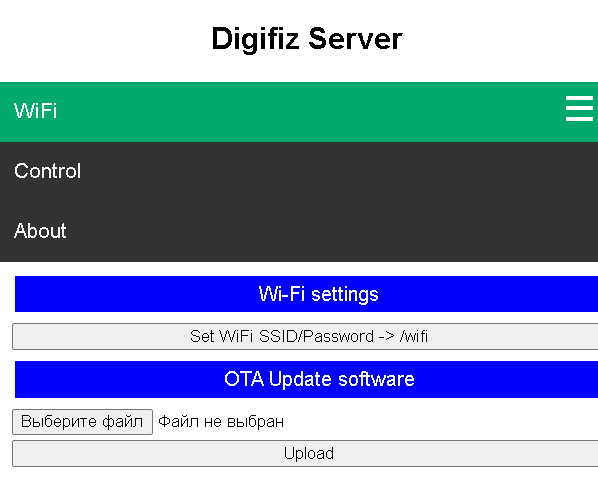
\includegraphics[width=\linewidth]{digifiz_manual/image020.png}
        \caption{Control tab overview.}
    \end{subfigure}\hfill
    \begin{subfigure}{0.48\textwidth}
        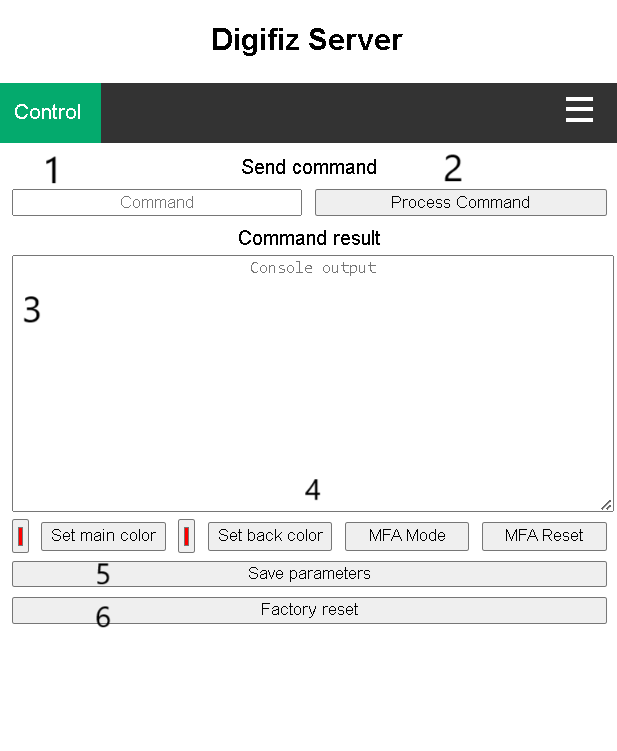
\includegraphics[width=\linewidth]{digifiz_manual/image021.png}
        \caption{Numbered controls and command entry fields.}
    \end{subfigure}
    \caption{\ReplicaNextShort{} Wi-Fi control interface.}
    \label{fig:next-control-tabs}
\end{figure}

\section{Command entry}
The \emph{Control} tab provides a command input line (1), a \emph{Process} button (2), a result window (3), quick controls (4), a \emph{Save} button (5), and a \emph{Reset} button (6). Enter commands as space-separated pairs \verb|<number> <value>| using integers only; punctuation and quotation marks are not required. \autoref{fig:next-command-example} illustrates the interface while toggling automatic brightness.

\begin{figure}[htbp]
    \centering
    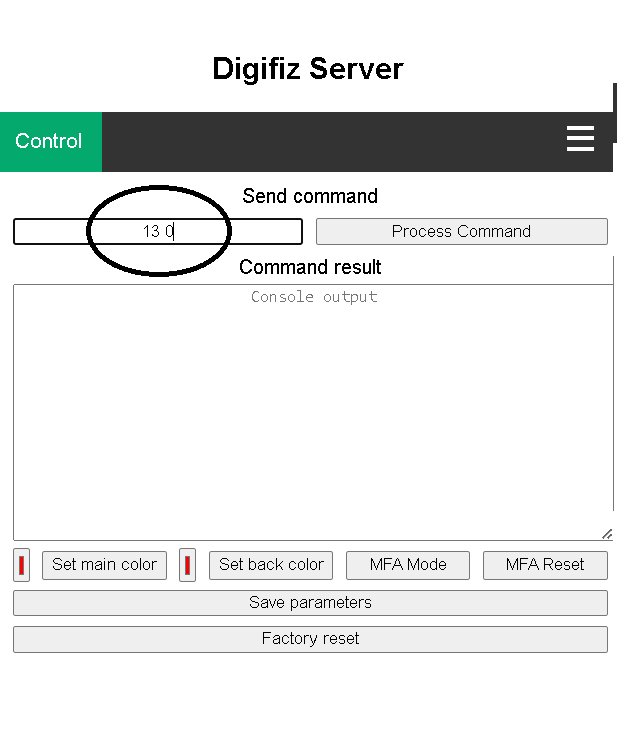
\includegraphics[width=0.55\textwidth]{digifiz_manual/image022.png}
    \caption{Example command sequence disabling automatic brightness.}
    \label{fig:next-command-example}
\end{figure}

\section{Command reference}
\begin{table}[htbp]
    \centering
    \caption{Primary \ReplicaNextShort{} configuration commands.}
    \label{tbl:next-commands}
    {\scriptsize
    \begin{tblr}{
        colspec = {Q[c,0.14\linewidth] Q[l,0.36\linewidth] Q[l]},
        rowsep = 2pt,
    }
        \toprule
        \textbf{Command} & \textbf{Name} & \textbf{Description} \\
        \midrule
        22 (or 0) & \paramname{PARAMETER\_RPMCOEFFICIENT} & Engine RPM calibration factor (100--10000). \\
        1  & \paramname{PARAMETER\_SPEEDCOEFFICIENT} & Speed calibration factor (10--255). \\
        2  & \paramname{PARAMETER\_COOLANTTHERMISTORB} & Coolant thermistor beta coefficient (2000--5000). \\
        3  & \paramname{PARAMETER\_OILTHERMISTORB} & Oil thermistor beta coefficient (2000--5000). \\
        4  & \paramname{PARAMETER\_AIRTHERMISTORB} & Ambient thermistor beta coefficient (2000--5000). \\
        5  & \paramname{PARAMETER\_TANKMINRESISTANCE} & Minimum fuel sender resistance (0--1000~\ohm). \\
        6  & \paramname{PARAMETER\_TANKMAXRESISTANCE} & Maximum fuel sender resistance (100--1000~\ohm). \\
        7  & \paramname{PARAMETER\_TAU\_COOLANT} & Coolant temperature filter constant (1--50, higher is more responsive). \\
        8  & \paramname{PARAMETER\_TAU\_OIL} & Oil temperature filter constant (1--50). \\
        9  & \paramname{PARAMETER\_TAU\_AIR} & Ambient temperature filter constant (1--50). \\
        10 & \paramname{PARAMETER\_TAU\_TANK} & Fuel level filter constant (1--50). \\
        11 & \paramname{PARAMETER\_MILEAGE} & Total odometer value (0--999999). \\
        12 & \paramname{PARAMETER\_DAILY\_MILEAGE} & Trip odometer (0--9999). \\
        13 & \paramname{PARAMETER\_AUTO\_BRIGHTNESS} & Automatic brightness enable (1=on, 0=off). \\
        14 & \paramname{PARAMETER\_BRIGHTNESS\_LEVEL} & Manual brightness level (0--60\%; values above 60 reduce LED life). \\
        15 & \paramname{PARAMETER\_TANK\_CAPACITY} & Fuel tank capacity in litres (0--99; 55~L typical for Golf~2). \\
        16 & \paramname{PARAMETER\_MFA\_STATE} & Active MFA mode (normally controlled via hardware input). \\
        17 & \paramname{PARAMETER\_BUZZER\_OFF} & Disable buzzer (1 disables, 0 enables; \ReplicaNextShort{} lacks a buzzer). \\
        18 & \paramname{PARAMETER\_MAX\_RPM} & Tachometer scaling (typical 8000, range 4000--16000). \\
        19 & \paramname{PARAMETER\_NORMAL\_RESISTANCE\_COOLANT} & Coolant sensor resistance at \SI{25}{\celsius} (1000--10000~\ohm). \\
        20 & \paramname{PARAMETER\_NORMAL\_RESISTANCE\_OIL} & Oil sensor resistance at \SI{25}{\celsius} (1000--10000~\ohm). \\
        21 & \paramname{PARAMETER\_NORMAL\_RESISTANCE\_AMB} & Ambient sensor resistance at \SI{25}{\celsius} (1000--10000~\ohm). \\
        23 & \paramname{PARAMETER\_DOT\_OFF} & Clock colon behaviour (0=blink, 1=solid). \\
        24 & \paramname{PARAMETER\_BACKLIGHT\_ON} & Enable backlight on low beam (not used on \ReplicaNextShort{}). \\
        25 & \paramname{PARAMETER\_M\_D\_FILTER} & Median filter constant (legacy, normally unused). \\
        26 & \paramname{PARAMETER\_COOLANT\_MAX\_R} & Coolant sensor threshold for full-scale indication (\SI{100}{\celsius}--\SI{150}{\celsius}). \\
        27 & \paramname{PARAMETER\_COOLANT\_MIN\_R} & Coolant sensor threshold for ``1~bar'' indication (\SI{0}{\celsius}--\SI{80}{\celsius}). \\
        31 & \paramname{PARAMETER\_MAINCOLOR\_R} & Red component of the UI colour (0--255). \\
        32 & \paramname{PARAMETER\_MAINCOLOR\_G} & Green component of the UI colour (0--255). \\
        33 & \paramname{PARAMETER\_MAINCOLOR\_B} & Blue component of the UI colour (0--255). \\
        37 & \paramname{PARAMETER\_RPM\_FILTER} & RPM filter aggressiveness (10--200, higher reacts faster). \\
        128 & \paramname{PARAMETER\_READ\_ADDITION} & Add 128 to read the current value of any command. \\
        255 & \paramname{PARAMETER\_SET\_HOUR} & Set clock hours (24-hour format). \\
        254 & \paramname{PARAMETER\_SET\_MINUTE} & Set clock minutes. \\
        253 & \paramname{PARAMETER\_RESET\_DAILY\_MILEAGE} & Reset the trip odometer. \\
        252 & \paramname{PARAMETER\_RESET\_DIGITAL} & Factory reset of stored parameters. \\
        \bottomrule
    \end{tblr}}
\end{table}

\section{Default values}
\begin{table}[htbp]
    \centering
    \caption{\ReplicaNextShort{} default settings.}
    \label{tbl:next-defaults}
    {\scriptsize
    \begin{tblr}{
        colspec = {Q[l,0.42\linewidth] Q[c,0.15\linewidth] Q[l]},
        rowsep = 2pt,
    }
        \toprule
        \textbf{Parameter} & \textbf{Default} & \textbf{Notes} \\
        \midrule
        \paramname{PARAMETER\_RPMCOEFFICIENT} & 3000 & Typical for Audi tachometer inputs. \\
        \paramname{PARAMETER\_SPEEDCOEFFICIENT} & 100 & Calibrated for 100~km/h. \\
        \paramname{PARAMETER\_COOLANTTHERMISTORB} & 4000 &  \\
        \paramname{PARAMETER\_OILTHERMISTORB} & 4000 &  \\
        \paramname{PARAMETER\_AIRTHERMISTORB} & 3812 & 3600 for Generation~2 panels. \\
        \paramname{PARAMETER\_TANKMINRESISTANCE} & 35 & \ohm. \\
        \paramname{PARAMETER\_TANKMAXRESISTANCE} & 265 & \ohm. \\
        \paramname{PARAMETER\_TAU\_COOLANT} & 2 & Filter constant. \\
        \paramname{PARAMETER\_TAU\_OIL} & 2 & Filter constant. \\
        \paramname{PARAMETER\_TAU\_AIR} & 2 & Filter constant. \\
        \paramname{PARAMETER\_TAU\_TANK} & 2 & Filter constant. \\
        \paramname{PARAMETER\_MILEAGE} & Vehicle-specific & Retains stored odometer. \\
        \paramname{PARAMETER\_DAILY\_MILEAGE} & 0 &  \\
        \paramname{PARAMETER\_AUTO\_BRIGHTNESS} & 1 & Enabled. \\
        \paramname{PARAMETER\_BRIGHTNESS\_LEVEL} & 25 & Generation~2 default; Generation~1/1.5 use 7 or 13. \\
        \paramname{PARAMETER\_TANK\_CAPACITY} & 63 & Litres. \\
        \paramname{PARAMETER\_MFA\_STATE} & 0 & Default MFA page. \\
        \paramname{PARAMETER\_BUZZER\_OFF} & 1 & Buzzer disabled. \\
        \paramname{PARAMETER\_MAX\_RPM} & 8000 & Tachometer scale. \\
        \paramname{PARAMETER\_NORMAL\_RESISTANCE\_COOLANT} & 1000 & \ohm{} at \SI{25}{\celsius}. \\
        \paramname{PARAMETER\_NORMAL\_RESISTANCE\_OIL} & 1000 & \ohm{} at \SI{25}{\celsius}. \\
        \paramname{PARAMETER\_NORMAL\_RESISTANCE\_AMB} & 2991 & 500~\ohm{} for Generation~2 sensors. \\
        \paramname{PARAMETER\_DOT\_OFF} & 0 & Blinking clock colon. \\
        \paramname{PARAMETER\_BACKLIGHT\_ON} & 1 & Backlight enabled with low beam. \\
        \paramname{PARAMETER\_M\_D\_FILTER} & 65535 & Legacy median filter constant. \\
        \paramname{PARAMETER\_COOLANT\_MAX\_R} & 120 & \si{\celsius}. \\
        \paramname{PARAMETER\_COOLANT\_MIN\_R} & 60 & \si{\celsius}. \\
        \paramname{PARAMETER\_MAINCOLOR\_R} & 180 & Yellow-green default. \\
        \paramname{PARAMETER\_MAINCOLOR\_G} & 240 & Yellow-green default. \\
        \paramname{PARAMETER\_MAINCOLOR\_B} & 6 & Yellow-green default. \\
        \paramname{PARAMETER\_RPM\_FILTER} & 70 & Filter response. \\
        \paramname{PARAMETER\_UPTIME} & 0 & Runtime counter. \\
        \bottomrule
    \end{tblr}}
\end{table}

\section{Reading parameters and examples}
To read a parameter, add 128 to the command number (for example, \verb|129 0| reports the speed coefficient). Typical commands include disabling automatic brightness (\verb|13 0|), enabling it again (\verb|13 1|), adjusting the speed coefficient (\verb|1 110| increases the displayed speed by 10\%), and setting the odometer (\verb|11 123456|). Clock values are set with \verb|255 <hours>| followed by \verb|254 <minutes>|. Commands 31--33 set the RGB components of the user interface colour.

\section{Service commands}
Recent firmware revisions accept human-readable parameter names, for example \verb|PARAMETER_RPMCOEFFICIENT 3000|. The diagnostic command \verb|adc 0| prints raw ADC readings for sensor troubleshooting. Firmware updates add visual colour controls, so update regularly through the \emph{WiFi} tab to access the latest features.

\section{Settings tab parameter editor}
The \emph{Settings} tab mirrors the parameter list in \autoref{tbl:next-commands} and \autoref{tbl:next-defaults} while adding metadata about ranges, descriptions, and data types.
Use it whenever you prefer a graphical workflow instead of typing command numbers.

\begin{enumerate}
    \item Press \emph{Load Parameters} to fetch the live values from the dashboard. The browser displays each item with its name, current value, tooltip, and type.
    \item For numeric entries, type the desired value inside the \emph{New Value} column. The interface enforces the permissible range shown in the \emph{Min} and \emph{Max} columns. Boolean parameters appear as checkboxes.
    \item Click \emph{Set} to submit the change instantly. The table refreshes to confirm the updated value.
    \item Repeat the process for every parameter you want to adjust. When finished, return to the \emph{Control} tab and press \emph{Save parameters} to write the configuration to non-volatile memory.
\end{enumerate}

The colour workflow requires that you enable the firmware flag responsible for custom palettes before moving to the \emph{Colors} tab.
Locate the boolean entry labelled ``Custom colour scheme'' (published as \verb|PARAMETER_CUSTOM_COLORSCHEME_ENABLE| in the parameter list), tick the checkbox, and press \emph{Set}. The dashboard will reject bespoke segment edits until this flag is turned on.

\section{Custom colour schemes}
The \emph{Colors} tab introduces a segment-based editor for the WS2812 LED backlight. Each row describes a range end point, the functional area it corresponds to, and the colour or base colour inheritance.

\begin{enumerate}
    \item Press \emph{Load Scheme} to read the active mapping. Use \emph{Add Segment}, or the inline ``+\textuparrow{}'' and ``+\textdownarrow{}'' controls, to insert new ranges. The drop-down menus select the instrument function, and the base-colour selector lets you reuse the main or back colours instead of specifying a fixed RGB value.
    \item Click the colour picker to fine-tune the RGB tone for segments that are set to ``Custom''. The editor reports component values in real time.
    \item Use the reorder arrows to match the physical LED sequence (segments must remain in ascending order). Delete redundant rows with the ``\texttimes{}'' button.
    \item When the table reflects the desired layout, press \emph{Set Scheme}. The browser iterates through the rows and pushes each segment to the dashboard.
    \item Immediately switch to the \emph{Control} tab and press \emph{Save parameters}. This step is mandatory---the firmware caches the uploaded segments in RAM and discards them after a reboot if they are not saved.
    \item Optionally export the JSON representation via \emph{Export to File} for backups, or import a previously saved file with \emph{Import from File}. The \emph{Reset Scheme} button restores the factory layout after confirmation.
\end{enumerate}

If you later disable the custom colour scheme flag in the \emph{Settings} tab, the dashboard falls back to the classic single-colour mode driven by \verb|PARAMETER_MAINCOLOR_R/G/B|.
